\documentclass{article}
\usepackage{graphicx}
\usepackage[margin=1.5cm]{geometry}
\usepackage{amsmath}

\begin{document}

\title{Wednesday Reading Assessment: Unit 6, Circular Motion}
\author{Prof. Jordan C. Hanson}

\maketitle

\section{Memory Bank}

\begin{itemize}
\item $\vec{F}_G = G \frac{m_1 m_2}{r^2} \hat{r}$
\item $G = 6.674 \times 10^{-11}$ N kg$^{-2}$ m$^2$
\end{itemize}

\section{Newton's Law of Gravity}

\begin{enumerate}
\item
\begin{figure}[ht]
\centering
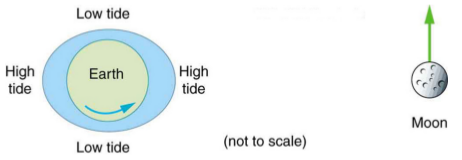
\includegraphics[width=0.45\textwidth]{tide1.png}
\caption{\label{fig:tide1} The tides of the Earth as they relate to the position of the Moon.}
\end{figure}
Explain in your own words why the high tides of the Earth's oceans orient themselves as in Fig. \ref{fig:tide1}.  Recall that Newton's Law of Gravity depends on $1/r^2$.  \\ \vspace{2cm}
\item The spring tides are the highest high tides, and the neap tides are the lowest high tides.  Explain why this is the case using Fig. \ref{fig:tide2} and Newton's Law of Gravity.
\begin{figure}[hb]
\centering
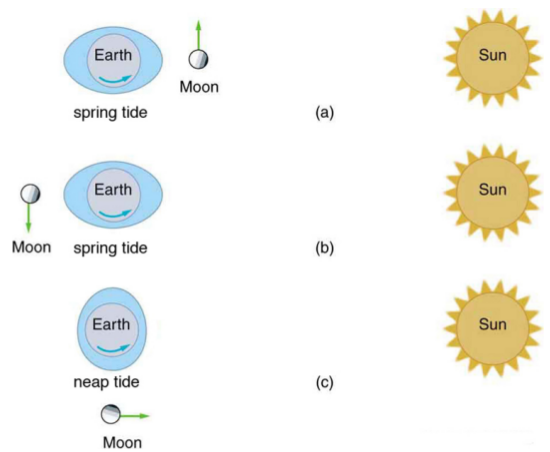
\includegraphics[width=0.4\textwidth]{tide2.png}
\caption{\label{fig:tide2} The spring and neap tides as they relate to the orientation of the Earth, Moon, and Sun.}
\end{figure}
\end{enumerate}

\end{document}
